\documentclass[journal]{IEEEtran}


% *** GRAPHICS RELATED PACKAGES ***
%
\ifCLASSINFOpdf
  % \usepackage[pdftex]{graphicx}
  % declare the path(s) where your graphic files are
  % \graphicspath{{../pdf/}{../jpeg/}}
  % and their extensions so you won't have to specify these with
  % every instance of \includegraphics
  % \DeclareGraphicsExtensions{.pdf,.jpeg,.png}
\else
  % or other class option (dvipsone, dvipdf, if not using dvips). graphicx
  % will default to the driver specified in the system graphics.cfg if no
  % driver is specified.
  % \usepackage[dvips]{graphicx}
  % declare the path(s) where your graphic files are
  % \graphicspath{{../eps/}}
  % and their extensions so you won't have to specify these with
  % every instance of \includegraphics
  % \DeclareGraphicsExtensions{.eps}
\fi
% graphicx was written by David Carlisle and Sebastian Rahtz. It is
% required if you want graphics, photos, etc. graphicx.sty is already
% installed on most LaTeX systems. The latest version and documentation
% can be obtained at: 
% http://www.ctan.org/pkg/graphicx
% Another good source of documentation is "Using Imported Graphics in
% LaTeX2e" by Keith Reckdahl which can be found at:
% http://www.ctan.org/pkg/epslatex
%
% latex, and pdflatex in dvi mode, support graphics in encapsulated
% postscript (.eps) format. pdflatex in pdf mode supports graphics
% in .pdf, .jpeg, .png and .mps (metapost) formats. Users should ensure
% that all non-photo figures use a vector format (.eps, .pdf, .mps) and
% not a bitmapped formats (.jpeg, .png). The IEEE frowns on bitmapped formats
% which can result in "jaggedy"/blurry rendering of lines and letters as
% well as large increases in file sizes.
%
% You can find documentation about the pdfTeX application at:
% http://www.tug.org/applications/pdftex



% *** ALIGNMENT PACKAGES ***
%
%\usepackage{array}
% Frank Mittelbach's and David Carlisle's array.sty patches and improves
% the standard LaTeX2e array and tabular environments to provide better
% appearance and additional user controls. As the default LaTeX2e table
% generation code is lacking to the point of almost being broken with
% respect to the quality of the end results, all users are strongly
% advised to use an enhanced (at the very least that provided by array.sty)
% set of table tools. array.sty is already installed on most systems. The
% latest version and documentation can be obtained at:
% http://www.ctan.org/pkg/array


% IEEEtran contains the IEEEeqnarray family of commands that can be used to
% generate multiline equations as well as matrices, tables, etc., of high
% quality.



% *** FLOAT PACKAGES ***
%
%\usepackage{fixltx2e}
% fixltx2e, the successor to the earlier fix2col.sty, was written by
% Frank Mittelbach and David Carlisle. This package corrects a few problems
% in the LaTeX2e kernel, the most notable of which is that in current
% LaTeX2e releases, the ordering of single and double column floats is not
% guaranteed to be preserved. Thus, an unpatched LaTeX2e can allow a
% single column figure to be placed prior to an earlier double column
% figure.
% Be aware that LaTeX2e kernels dated 2015 and later have fixltx2e.sty's
% corrections already built into the system in which case a warning will
% be issued if an attempt is made to load fixltx2e.sty as it is no longer
% needed.
% The latest version and documentation can be found at:
% http://www.ctan.org/pkg/fixltx2e


%\usepackage{stfloats}
% stfloats.sty was written by Sigitas Tolusis. This package gives LaTeX2e
% the ability to do double column floats at the bottom of the page as well
% as the top. (e.g., "\begin{figure*}[!b]" is not normally possible in
% LaTeX2e). It also provides a command:
%\fnbelowfloat
% to enable the placement of footnotes below bottom floats (the standard
% LaTeX2e kernel puts them above bottom floats). This is an invasive package
% which rewrites many portions of the LaTeX2e float routines. It may not work
% with other packages that modify the LaTeX2e float routines. The latest
% version and documentation can be obtained at:
% http://www.ctan.org/pkg/stfloats
% Do not use the stfloats baselinefloat ability as the IEEE does not allow
% \baselineskip to stretch. Authors submitting work to the IEEE should note
% that the IEEE rarely uses double column equations and that authors should try
% to avoid such use. Do not be tempted to use the cuted.sty or midfloat.sty
% packages (also by Sigitas Tolusis) as the IEEE does not format its papers in
% such ways.
% Do not attempt to use stfloats with fixltx2e as they are incompatible.
% Instead, use Morten Hogholm'a dblfloatfix which combines the features
% of both fixltx2e and stfloats:
%
% \usepackage{dblfloatfix}
% The latest version can be found at:
% http://www.ctan.org/pkg/dblfloatfix




%\ifCLASSOPTIONcaptionsoff
%  \usepackage[nomarkers]{endfloat}
% \let\MYoriglatexcaption\caption
% \renewcommand{\caption}[2][\relax]{\MYoriglatexcaption[#2]{#2}}
%\fi
% endfloat.sty was written by James Darrell McCauley, Jeff Goldberg and 
% Axel Sommerfeldt. This package may be useful when used in conjunction with 
% IEEEtran.cls'  captionsoff option. Some IEEE journals/societies require that
% submissions have lists of figures/tables at the end of the paper and that
% figures/tables without any captions are placed on a page by themselves at
% the end of the document. If needed, the draftcls IEEEtran class option or
% \CLASSINPUTbaselinestretch interface can be used to increase the line
% spacing as well. Be sure and use the nomarkers option of endfloat to
% prevent endfloat from "marking" where the figures would have been placed
% in the text. The two hack lines of code above are a slight modification of
% that suggested by in the endfloat docs (section 8.4.1) to ensure that
% the full captions always appear in the list of figures/tables - even if
% the user used the short optional argument of \caption[]{}.
% IEEE papers do not typically make use of \caption[]'s optional argument,
% so this should not be an issue. A similar trick can be used to disable
% captions of packages such as subfig.sty that lack options to turn off
% the subcaptions:
% For subfig.sty:
% \let\MYorigsubfloat\subfloat
% \renewcommand{\subfloat}[2][\relax]{\MYorigsubfloat[]{#2}}
% However, the above trick will not work if both optional arguments of
% the \subfloat command are used. Furthermore, there needs to be a
% description of each subfigure *somewhere* and endfloat does not add
% subfigure captions to its list of figures. Thus, the best approach is to
% avoid the use of subfigure captions (many IEEE journals avoid them anyway)
% and instead reference/explain all the subfigures within the main caption.
% The latest version of endfloat.sty and its documentation can obtained at:
% http://www.ctan.org/pkg/endfloat
%
% The IEEEtran \ifCLASSOPTIONcaptionsoff conditional can also be used
% later in the document, say, to conditionally put the References on a 
% page by themselves.






% correct bad hyphenation here
\hyphenation{op-tical net-works semi-conduc-tor}
\usepackage{amsmath}
\usepackage{graphicx}
\usepackage{algorithmic}
\usepackage{url}
\usepackage{cite}
\usepackage[caption=false,font=footnotesize]{subfig}
%\usepackage{array}
\usepackage{amsmath}
\usepackage{pifont}


\newsavebox{\ieeealgbox}
\newenvironment{boxedalgorithmic}
  {\begin{lrbox}{\ieeealgbox}
   \begin{minipage}{\dimexpr\columnwidth-2\fboxsep-2\fboxrule}
   \begin{algorithmic}}
  {\end{algorithmic}
   \end{minipage}
   \end{lrbox}\noindent\fbox{\usebox{\ieeealgbox}}}


\makeatletter
\newcommand*{\rom}[1]{\expandafter\@slowromancap\romannumeral #1@}

\begin{document}
\title{A Strategy to Build Connection with a Stranger Based on Social Network Topology}
\author{Shaojun Zhang, ~\IEEEmembership{Department of Statistics,~University of Florida}}
\maketitle


\begin{abstract}
As we know, people are connected in various social networks such as phone calls, emails and Facebook. Then an interesting question arises whether we can improve our chance of making friends with some particular stranger in the network? Here the stranger can be our potential spouse, colleague, advisor or boss. Of course we can directly make a phone call, send an email or send an invitation through Facebook to the stranger. But we are very likely to be ignored or reported since we are completely unknown to the stranger. Moreover, private information such as email addresses and phone numbers are unavailable most of time.

One straightforward solution is to link one by one along the shortest path to the target. However, the problem becomes complicated when the shortest path is still long or when there exists more than one shortest path, especially in a dense network. In this report, I develop a strategy based on network topology including shortest paths, community structure and eigenvector centrality to deal with these problems. The method and the accompanying analysis will be illustrated on a dataset covering email communication of about 150 users of Enron, an American energy company.
\end{abstract}


\section{Introduction}
\IEEEPARstart{N}{owadays}, people have many ways to communicate with each other. We can make phone calls, write text messages, send emails as well as send messages online via websites or applets. All of these communications forms our social network. 

An interesting problem is that if we have access to the network data, how we can benefit ourselves by building connection with some stranger that we are interested. For example, the stranger can be our potential advisor that we find on the department website when applying for a PhD program. There are many more such examples and this situation is very common.

Obviously, if there is a path between the stranger and me in the network, there must be a direct friend of mine on the path. Therefore, I can ask him or her to introduce the next person on the path to me. In this way, I can make friends one by one along the path until I reach the stranger. If there are many paths to the stranger, we will of course choose the shortest one. But what if there are still many shortest paths? Also, we may not be willing to keep connecting if the path is long.

In this report, I proposed a strategy that combines community structure, eigenvector centrality and some other criteria to deal with these problems. I set an upper bound for the number of people allowed to link and use it to truncate all shortest paths. All comparisons among candidate paths are based on these truncated paths. Louvain method and label propagation algorithm are used for community detection. Two versions of community score and an importance score are defined and used for path selection.

The outline of the report is as follows. In Sec. \rom{2}, I describe the basic characteristics of the Enron network, some assumptions needed and the detailed method. In Sec. \rom{3}, I give and analyze the main results. In Sec. \rom{4}, I describe several algorithms related to my strategy. In Sec. \rom{5}, I give my conclusions, remaining problems and possible extensions.


\section{Description}
\subsection{Data}
The Enron email dataset \cite{Klimt:2004aa} was collected and prepared by the CALO project. It contains data from about 150 users, mostly senior management of Enron organized into folders. This data was originally made public, and posted to the web, by the Federal Energy Regulatory Commission during its investigation. This data is valuable because it is the only substantial collection of ``real" email that is public \cite{:ac}. 

The network formed by these email communications is a typical social network. Its properties may be very different from those of other types of social network such as phone calls. But the method in this report can be applied to all networks including large datasets such as Facebook or Twitter.

The undirected graph induced by the entire Enron email dataset contains 36692 vertices and 183831 edges. Unfortunately, it is not a connected graph, which means that there does not exist a path between some pairs of users. Therefore, these pairs of users cannot become friends based on the information from the email communications. 

However, we can focus on connected components so that any two users in each component are linked by at least one path. Among all connected components, there is a giant component which contains $N_{v} = 33696$ vertices and $N_{e} = 180811$ edges, covering 92\% vertices and 98\% edges respectively in the whole graph as shown in Fig. \ref{fig:1}. Therefore, all the analysis and results below are based on the giant component instead of the whole graph.

\begin{figure*}[!t]
\centering
\subfloat[]{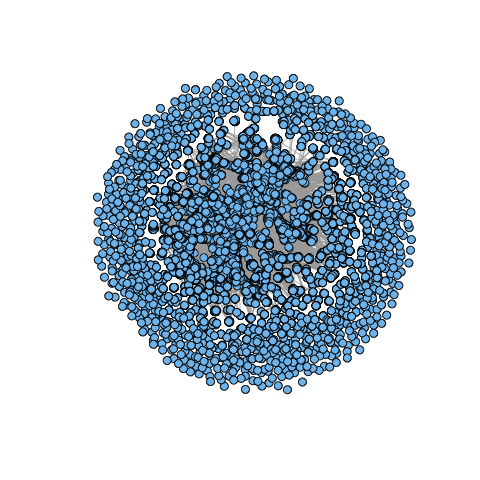
\includegraphics[width=2.5in]{../Images/whole_graph.png} \label{fig:1a}}
\hfil
\subfloat[]{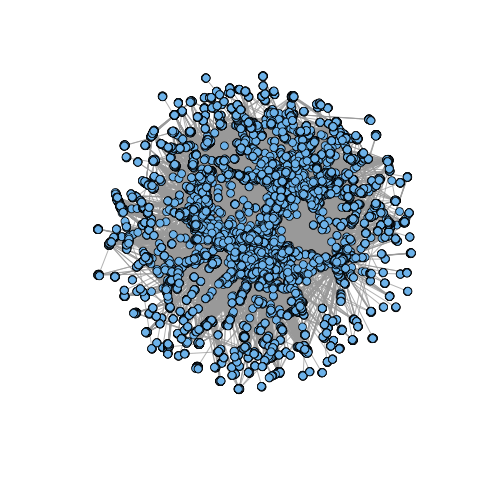
\includegraphics[width=2.5in]{../Images/giant_graph.png} \label{fig:1b}}
\caption{The network of the Enron email communication. \protect\subref{fig:1a} is the whole graph and \protect\subref{fig:1b} is the subgraph of the giant component.}
\label{fig:1}
\end{figure*}

The diameter of the graph is 13 and the average path length of the graph is 4.02. According to the well-known six degrees of separation theory, everyone and everything is six or fewer steps away, by way of introduction, from any other person in the world \cite{Barabasi:2003aa}. Therefore, the average distance between users in the Enron network is shorter than that in our real world. The Enron network may even be a small-world network \cite{D.-J.-Watts:1998aa}. 

The average degree of the graph is 10.73 and the average clustering coefficient of the graph is 0.71. To see the degree behavior for all vertices in the graph, a power law distribution with two parameters is fitted. 

First the probability density function of degree is assumed to be $f_{d} = C  d^{- \alpha}$ for $d$ in $[x_{min}, \infty)$, where $C$ is a constant. After integrating both sides with respect to $d$, we have $C = (\alpha - 1) x_{min}^{\alpha - 1}$. Thus the density function becomes 
$$f_{d} =  \frac{\alpha - 1}{x_{min}} \left( \frac{d}{x_{min}} \right)^{- \alpha}.$$
After taking the log of both sides, we have a linear form 
$$\log f_{d} = \log(\alpha - 1) + (\alpha - 1) \log x_{min} - \alpha \log d,$$
which seems suitable for the Enron dataset as shown in Fig. \ref{fig:2}. The two parameters are estimated using maximum likelihood and we have $\hat{\alpha} = 1.98$ and $\widehat{x_{min}} = 5$.

\begin{figure}[!t]
\centering
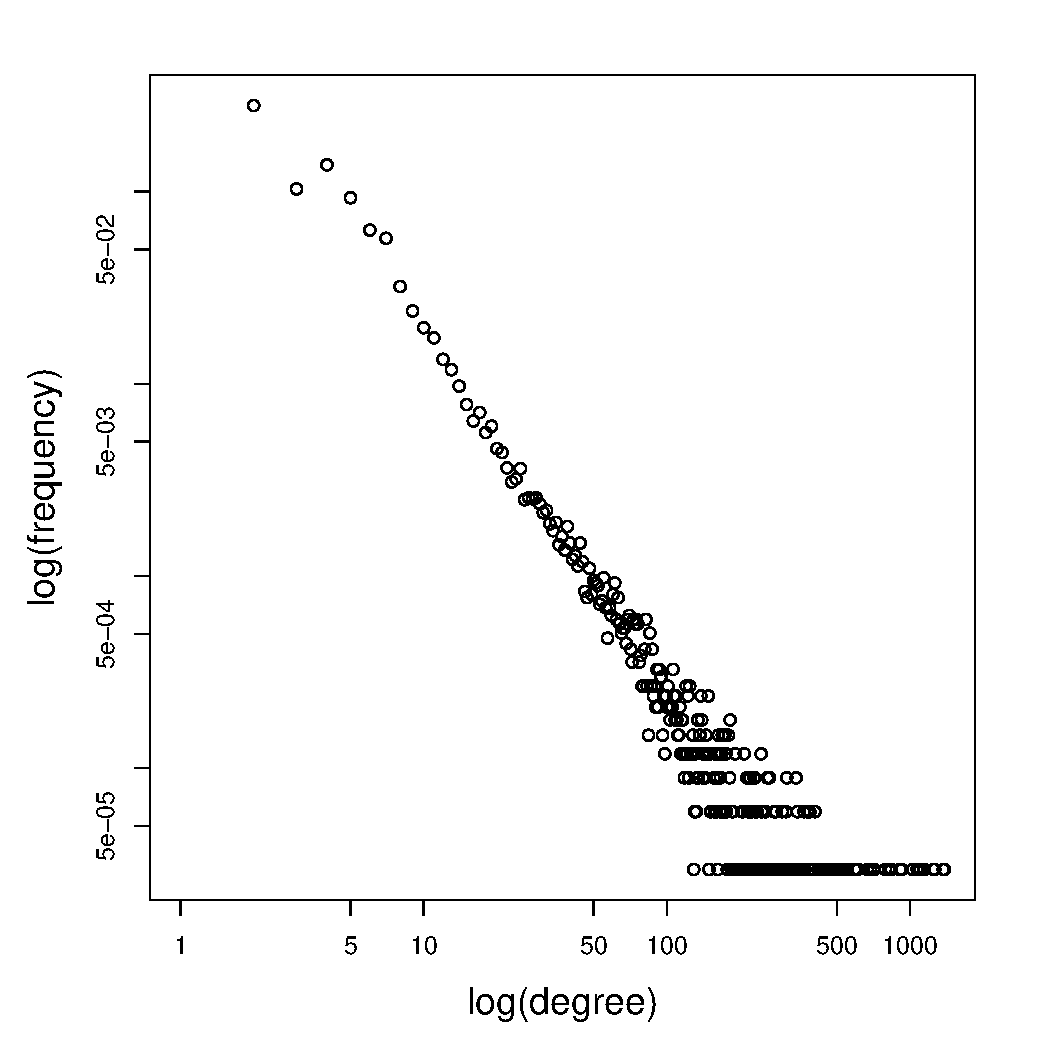
\includegraphics[width=2.5in]{../Images/degree_distribution.pdf}
\caption{Degree distribution.}
\label{fig:2}
\end{figure}

Closeness centrality, betweenness centrality and eigenvector centrality for all vertices are calculated. Top 10 vertices with highest scores for each type of centrality are compared and shown in Table \ref{tab:1}. The results of closeness centrality and eigenvector centrality are similar while the results of betweenness centrality are much different. 

\begin{table}[h]
\renewcommand{\arraystretch}{1.3}
\centering
\caption{Top 10 vertices for three centralities}
\label{tab:1}
\begin{tabular}{| c |  c | c | c |}
\hline
Rank & Closeness & Betweenness & Eigenvector \\
\hline
1 & 137 & 5025 & 137\\
2 & 77 & 141 & 196\\
3 & 47 & 567 & 77\\
4 & 141 & 589 & 371\\   
5 & 371 & 1140 & 1029\\    
6 & 293 & 274 & 274\\      
7 & 196 & 459 & 735\\     
8 & 735 & 47 & 417\\
9 & 176 & 1029 & 176\\
10 & 417 & 293 & 293\\
\hline
\end {tabular}
\end{table}

\subsection{Assumptions}
To establish the method, I make the following assumptions: 

\begin{enumerate}
\item\label{enu:1}
Friendships are based on edges in the graph and each user can only make new friends by being introduced. Since the network dataset is all we have, we can only deduce friendships and possible communications among users from the network topology. 
\item\label{enu:2}
Users in the same community have a closer relationship than those from different communities. By the definition of community, a vertex in a community is densely connected to other vertices in the same community, and sparsely connected to vertices outside the community. Therefore, in our case two users in the same community are likely to share more common friends and have more common interests.
\item\label{enu:3}
The more importance a user has, the more likely his or her friends will be introduced successfully. This assumption is motivated by the fact that if a user has a large influence, his or her friends will be more willing to accept or believe what the user says.
\item\label{enu:4}
Each user can only make at most 3 new friends excluding his or her direct friends. If the stranger becomes a friend of the user, the connection is built successfully. This restriction is based on the fact that each link has cost in the form of time, money or something else. 
\item
The network is fixed. That is to say, even if some user has made new friends, the network will remain unchanged. This assumption is made for simplicity. If several edges are added to a large network, its topology usually will not change much. What's more, while one user is making new friends, the relationships among other users are changing as well.
\end{enumerate}

\subsection{Method}
To apply the method, we need to choose two users, one as the user who is going to connect and the other as the stranger. They can be any two users in the network. After that, there are three steps to find the ``best'' path between them.

The first step is to find all shortest paths. Common shortest path algorithm such as Dijkstra's algorithm can only find one shortest path. Therefore, Yen's algorithm is used here to find $K$-shortest paths. As long as $K$ is large enough, we can find all shortest paths in the graph. For the Enron network, $K$ is chosen to be 10.

If the length of shortest paths $d \le 4$, the user can reach the stranger successfully according to Assumption \ref{enu:1} and Assumption \ref{enu:4}. Otherwise, the stranger is not reachable. In this case, the problem of the user becomes how to get as close as possible to the stranger so that the user can obtain a largest amount of possible information and may find other ways to reach the stranger. Since the user can reach at most 4 users on the path, all shortest paths are truncated if $d > 4$.

Next, I consider the community structure in the graph. Louvain method and label propagation algorithm are used for community detection. Two versions of community score are defined as follows:
\begin{equation*}
\begin{split}
C_{1} = \ &\mbox{number of pairs of neighboring users on the path}\\
&  \mbox{that belong to the same community},\\
C_{2} =\ & \mbox{number of users on the path that belong to the}\\
& \mbox{community containing the stranger}.
\end{split}
\end{equation*}
By Assumption \ref{enu:2}, a high community score indicates a high probability of connecting the stranger successfully. Therefore, the paths with highest community score ($C_{1}$ or $C_{2}$) are selected as further candidates. 

The importance of users in the network is used for final decision. An importance score is defined as follows:
\begin{equation*}
I = \mbox{ total eigenvector centrality scores on the path}.
\end{equation*}
By Assumption \ref{enu:3}, a high importance score also indicates a high probability of successful connections. Therefore, the path with highest importance score ($I$) is selected as the best path.

If there is only one path left after the first or the second step, the path is picked as the best path. If there are more than one path left after the last step, the best path is chosen randomly from them. The algorithm is as follows.

\begin{boxedalgorithmic}
\STATE Select all shortest paths using Yen's algorithm.
\IF{$d > 4$} \STATE{All shortest paths are truncated to first four vertices.} \ENDIF
\IF{only one path left} \STATE{Return the path.} \ELSE
\STATE Detect communities using Louvain method or label propagation and select the paths with largest $C_{i}, \ i = 1 \mbox{ or } 2$.
\IF{only one path left} \STATE{Return the path.} \ELSE \STATE{Compute eigenvector centrality scores and return the path with largest $I$.} \ENDIF
\ENDIF
\end{boxedalgorithmic}

\section{Evaluation}
For community detection, 239 communities are found by Louvain method and 903 by label propagation algorithm. Fig. \ref{fig:3} shows the distribution of community sizes for these two methods. Most communities found by label propagation algorithm contain a very small number of users.

\begin{figure*}[!t]
\centering
\subfloat[]{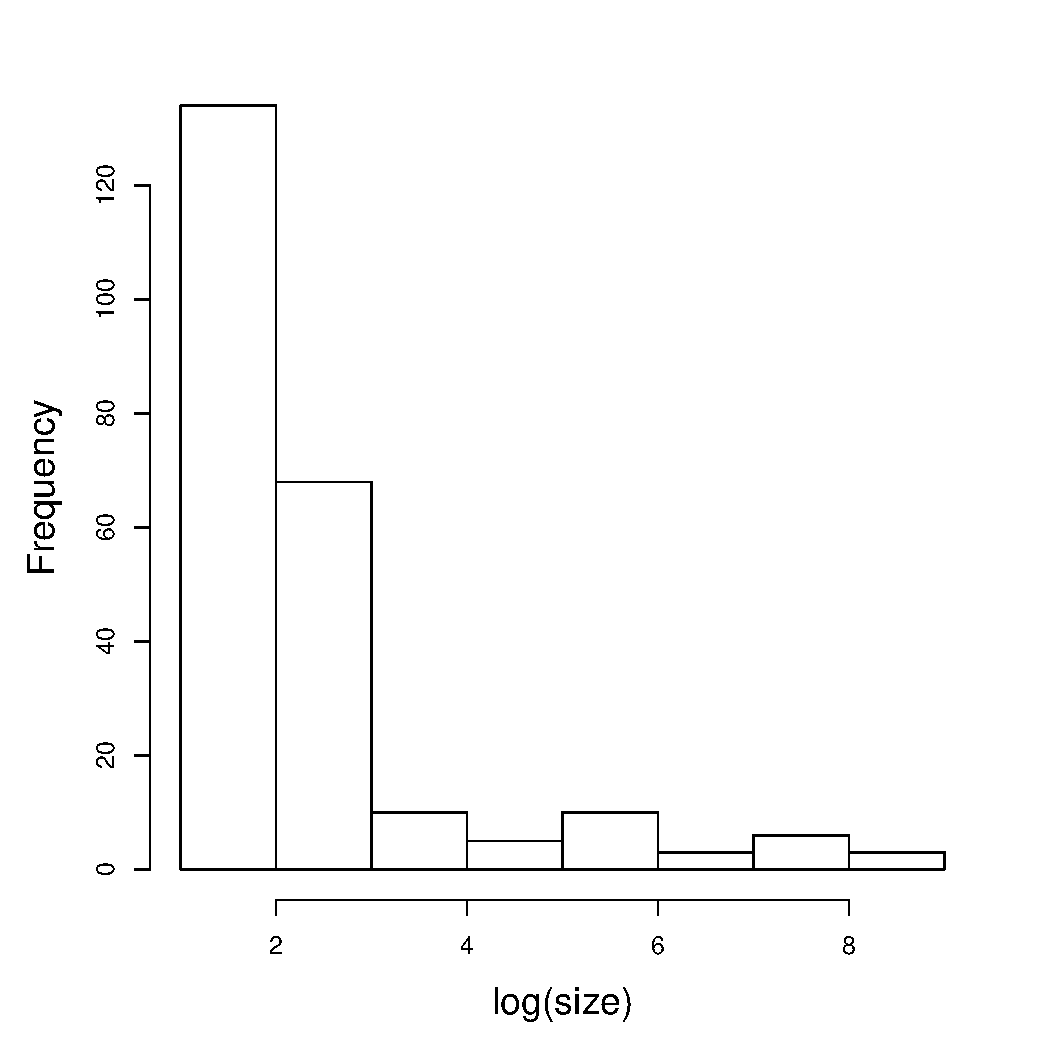
\includegraphics[width=2.5in]{../Images/hist_community_louvain.pdf} \label{fig:3a}}
\hfil
\subfloat[]{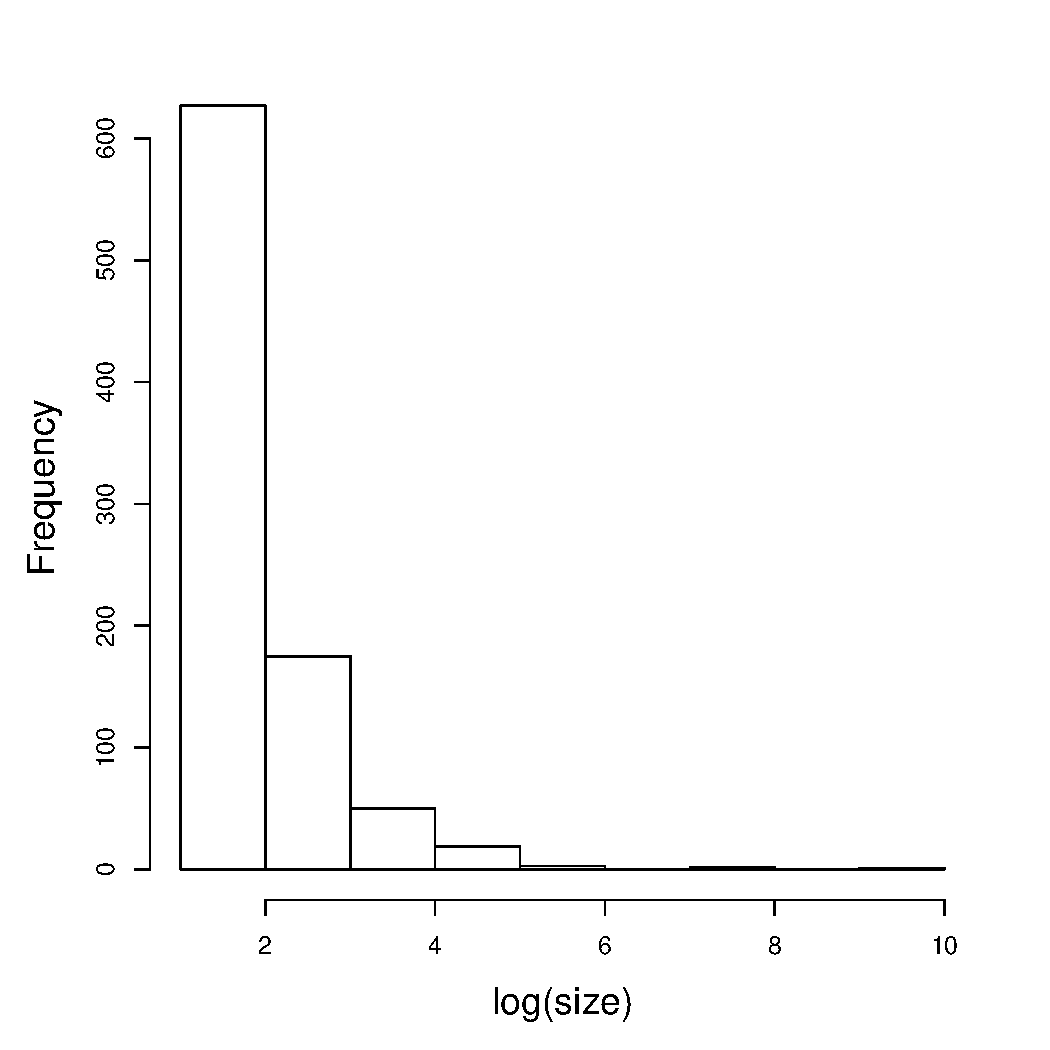
\includegraphics[width=2.5in]{../Images/hist_community_label.pdf} \label{fig:3b}}
\caption{Distribution of community sizes for \protect\subref{fig:3a} Louvain method and \protect\subref{fig:3b} label propagation algorithm.}
\label{fig:3}
\end{figure*}

10 pairs of users are randomly sampled from the network with the restriction that the two users in any pair belong to different communities. The restriction is made to bring some challenge to connections and to resemble real-life situations when we are interested in linking someone who is not close to us. 

The results are presented in Table \ref{tab:2} and Table \ref{tab:3}. In these two tables, the first two columns contain the indices of users who are going to connect and the indices of strangers. SP$\#$ means the number of shortest paths between two users. Column $C_{1}$ and $C_{2}$ contain the best paths found with community score defined as $C_{1}$ and $C_{2}$ respectively. Success indicates whether the user has build connection with the stranger successfully.

All pairs of users in the samples are connected by more than one shortest path, which justifies the necessity of path selection. Besides, a large proportion of connections are successful within limited linking steps. The best paths picked by using $C_{1}$ are mostly the same as those picked by using $C_{2}$, suggesting that the two statistics may have a positive correlation.

\begin{table*}[h]
\renewcommand{\arraystretch}{1.3}
\centering
\caption{Results when Louvain method is used for community detection}
\label{tab:2}
\begin{tabular}{| c | c | c | c | c | c |}
\hline
From & To & SP$\#$ & $C_{1}$ & $C_{2}$ & Success\\
\hline
17085 & 9609 & 7 & 17085 $\rightarrow$ 1029 $\rightarrow$ 2287 $\rightarrow$ 2295 $\rightarrow$ 9609 & 17085 $\rightarrow$ 274 $\rightarrow$ 77 $\rightarrow$ 343 $\rightarrow$ 9609 & \ding{51}\\
12885 & 27890 & 5  &  12885 $\rightarrow$ 274 $\rightarrow$ 10 $\rightarrow$8543 $\rightarrow$ 27890 & 12885 $\rightarrow$ 274 $\rightarrow$ 10 $\rightarrow$ 8543 $\rightarrow$ 27890 & \ding{51}\\
32349 & 20592 & 4  & 32349 $\rightarrow$ 14051 $\rightarrow$ 1140 $\rightarrow$  77 $\rightarrow$ 1589 & 32349 $\rightarrow$ 14051 $\rightarrow$ 1140 $\rightarrow$  274 $\rightarrow$ 1589 & \ding{55}\\
1764 & 12172 & 7  & 1764 $\rightarrow$ 96 $\rightarrow$ 12172 & 1764 $\rightarrow$ 96 $\rightarrow$ 12172 & \ding{51}\\
11412 & 2063 & 5  & 11412 $\rightarrow$ 233 $\rightarrow$ 482 $\rightarrow$ 2063 & 11412 $\rightarrow$ 233 $\rightarrow$ 482 $\rightarrow$ 2063 & \ding{55}\\
8270 & 25406 & 3  & 8270 $\rightarrow$  75 $\rightarrow$ 57 $\rightarrow$ 10 $\rightarrow$ 5007 &  8270 $\rightarrow$  75 $\rightarrow$ 57 $\rightarrow$ 10 $\rightarrow$ 5007 & \ding{55}\\
7156 & 11071 & 4  &  7156 $\rightarrow$ 196 $\rightarrow$ 4026 $\rightarrow$11071 & 7156 $\rightarrow$ 196 $\rightarrow$ 442 $\rightarrow$11071 & \ding{51}\\
19878 & 19567 & 4  &  19878 $\rightarrow$ 1769 $\rightarrow$  152 $\rightarrow$ 4397 $\rightarrow$ 19567 & 19878 $\rightarrow$ 1769 $\rightarrow$  152 $\rightarrow$ 4397 $\rightarrow$ 19567 & \ding{51}\\
24041 & 16112 & 4  & 24041 $\rightarrow$ 287 $\rightarrow$ 424 $\rightarrow$  226 $\rightarrow$ 16112 & 24041 $\rightarrow$ 287 $\rightarrow$ 79 $\rightarrow$  226 $\rightarrow$ 16112 & \ding{51}\\
12405 & 7156 & 6  & 12405 $\rightarrow$ 459 $\rightarrow$ 196 $\rightarrow$ 7156 & 12405 $\rightarrow$ 459 $\rightarrow$ 196 $\rightarrow$ 7156 & \ding{51}\\
\hline
\end{tabular}
\end{table*}

\begin{table*}[h]
\renewcommand{\arraystretch}{1.3}
\centering
\caption{Results when label propagation is used for community detection}
\label{tab:3}
\begin{tabular}{| c | c | c | c | c | c |}
\hline
From & To & SP$\#$ & $C_{1}$ & $C_{2}$ & Success\\
\hline
17085 & 20387 & 5 & 17085 $\rightarrow$ 1029 $\rightarrow$ 28 $\rightarrow$ 5020 $\rightarrow$ 20387 & 17085 $\rightarrow$ 1029 $\rightarrow$ 28 $\rightarrow$ 5020 $\rightarrow$ 20387 & \ding{51}\\
12885 & 31330 & 7 & 12885 $\rightarrow$ 274 $\rightarrow$ 10 $\rightarrow$ 5574 $\rightarrow$ 31330 & 12885 $\rightarrow$ 274 $\rightarrow$ 10 $\rightarrow$ 5574 $\rightarrow$ 31330 & \ding{51}\\
32349 & 20591 & 4 & 32349 $\rightarrow$ 14051 $\rightarrow$ 1140 $\rightarrow$ 77 $\rightarrow$ 1589 & 32349 $\rightarrow$ 14051 $\rightarrow$ 1140 $\rightarrow$ 77 $\rightarrow$ 1589 & \ding{55}\\
1764 & 22177 & 5 & 1764 $\rightarrow$ 214 $\rightarrow$ 823 $\rightarrow$ 22177 & 1764 $\rightarrow$ 293 $\rightarrow$ 3126 $\rightarrow$ 22177 & \ding{51}\\
11412 & 4662 & 5 & 11412 $\rightarrow$ 233 $\rightarrow$ 79 $\rightarrow$ 102 $\rightarrow$ 4662 & 11412 $\rightarrow$ 233 $\rightarrow$ 79 $\rightarrow$ 102 $\rightarrow$ 4662 & \ding{51}\\
8270 & 29942 & 4 & 8270 $\rightarrow$ 75 $\rightarrow$ 567 $\rightarrow$ 5025 $\rightarrow$ 29942 & 8270 $\rightarrow$ 75 $\rightarrow$ 567 $\rightarrow$ 5025 $\rightarrow$ 29942 & \ding{51}\\
7156 & 20152 & 5 & 7156 $\rightarrow$ 1140 $\rightarrow$ 7978 $\rightarrow$ 20152 & 7156 $\rightarrow$ 1140 $\rightarrow$ 7978 $\rightarrow$ 20152 & \ding{51}\\
19878 & 27221 & 4 & 19878 $\rightarrow$ 1769 $\rightarrow$ 1341 $\rightarrow$ 4151 $\rightarrow$ 27221 & 19878 $\rightarrow$ 1769 $\rightarrow$ 1341 $\rightarrow$ 4151 $\rightarrow$ 27221 & \ding{51}\\
24041 & 23720 & 4 & 24041 $\rightarrow$ 287 $\rightarrow$ 648 $\rightarrow$ 3310 $\rightarrow$ 23720 & 24041 $\rightarrow$ 287 $\rightarrow$ 517 $\rightarrow$ 3310 $\rightarrow$ 23720 & \ding{51}\\
12405 & 17544 & 5 & 12405 $\rightarrow$ 459 $\rightarrow$ 77 $\rightarrow$ 274 $\rightarrow$ 17544 & 12405   459    77   274 17544 & \ding{51}\\
\hline
\end{tabular}
\end{table*}

\section{Related work}
\subsection{Yen's algorithm}
Yen's algorithm \cite{Yen:1971aa} computes single-source $K$-shortest loopless paths for a graph with non-negative edge cost. The algorithm was published by Jin Y. Yen in 1971 and employs any shortest path algorithm to find the best path, then proceeds to find $K - 1$ deviations of the best path. 

Yen’s algorithm is known to be the efficient and widely used algorithm for determining $K$-shortest loopless paths \cite{Nagubadi:2013aa}. Its time complexity at worst case is $O(KN_{v}(N_{e} + N_{v} \log N_{v}))$ \cite{Labourdette:2006:PRM:1212284}.

\subsection{Louvain method}
The Louvain method \cite{1742-5468-2008-10-P10008} for community detection is a method to extract communities from large networks created by Vincent Blondel, Jean-Loup Guillaume, Renaud Lambiotte and Etienne Lefebvre. It is today one of the most widely used method for detecting communities in large networks. 

The method consists of two phases. 
\begin{itemize}
\item Phase 1: it looks for ``small'' communities by optimizing modularity in a local way. 
\item Phase 2: it aggregates nodes of the same community and builds a new network whose nodes are the communities. 
\item These two phases are repeated iteratively until a maximum of modularity is attained.
\end{itemize}

The advantage of Louvain method lies in its time complexity, which is $O(N_{v}^{2})$ for a general graph and $O(N_{v})$ for a sparse graph. However, the solution depends on the order of which node or community is to be selected for evaluating the modularity value in Phase 1
since it is a greedy method.

\subsection{Label propagation}
The key idea of label propagation algorithm \cite{PhysRevE.76.036106} is that each node finds a neighboring community of largest size to join until the system reaches equilibrium. Its time complexity is $O(N_{v})$.

In comparison with other algorithms, such as Newman's eigenvector method \cite{citeulike:646478}, label propagation has advantage in its running time, amount of a priori information needed about the network structure (no parameter is required to be known beforehand) while its disadvantage is that it produces no unique solution, but an aggregate of many solutions.

\section{Summary and Conclusions}
The strategy in this report combines community structure and eigenvector centrality to deal with multiple shortest paths. Two versions of community score and one importance score are defined as criteria for path selection. The assumptions made are reasonable and the method works well for the Enron email dataset. 

Since there is no ground truth or related social experiments, it is difficult for us to evaluate the strategy or compare it with other methods. The upper bound for the number of users allowed to link is chosen subjectively. I choose 3 here based on my personal experience.

Friendship in real life is much more complicated. Sometimes people are not willing to share their friends for various reasons. Moreover, friendship may change over time. A friend today may not be a friend tomorrow. Therefore, an interesting problem is how to find the best path in a dynamic network. Another interesting problem is how to integrate multiple social networks, for example, Facebook and Twitter.

The computer program for this project is written in R with igraph package. All computations for the report, including plotting, cost about 22.5 minutes on my laptop (2.5 GHz Intel Core i5, 4 GB 1600 MHz DDR3).




% Note that the IEEE does not put floats in the very first column
% - or typically anywhere on the first page for that matter. Also,
% in-text middle ("here") positioning is typically not used, but it
% is allowed and encouraged for Computer Society conferences (but
% not Computer Society journals). Most IEEE journals/conferences use
% top floats exclusively. 
% Note that, LaTeX2e, unlike IEEE journals/conferences, places
% footnotes above bottom floats. This can be corrected via the
% \fnbelowfloat command of the stfloats package.



% Can use something like this to put references on a page
% by themselves when using endfloat and the captionsoff option.
\ifCLASSOPTIONcaptionsoff
  \newpage
\fi

\IEEEtriggeratref{5}

% trigger a \newpage just before the given reference
% number - used to balance the columns on the last page
% adjust value as needed - may need to be readjusted if
% the document is modified later
%\IEEEtriggeratref{8}
% The "triggered" command can be changed if desired:
%\IEEEtriggercmd{\enlargethispage{-5in}}


\nocite{*}
\bibliographystyle{IEEEtran}
\bibliography{report}


\end{document}


